\documentclass{article}

\usepackage[a4paper]{geometry}
\usepackage[T1]{fontenc}
\usepackage{graphicx}
\usepackage{amsmath}
\usepackage{amssymb}
\usepackage{listings}
\usepackage{xcolor}
\usepackage{booktabs}
\usepackage{parskip}
\usepackage{float}

\definecolor{black}{HTML}{282828}
\definecolor{gray}{HTML}{928374}
\definecolor{red}{HTML}{cc241d}
\definecolor{green}{HTML}{98971a}
\definecolor{blue}{HTML}{458588}
\colorlet{background-color}{gray!5}

\lstset{
    basicstyle=\color{black}\ttfamily,
    keywordstyle=\color{red},
    commentstyle=\color{blue},
    stringstyle=\color{green},
    numberstyle=\color{black!35}\ttfamily,
    showspaces=false,
    showstringspaces=false,
    showtabs=false,
    columns=fullflexible,
    breaklines=true,
    postbreak=\mbox{\textcolor{gray}{\(\hookrightarrow\)}\space},
    escapechar=\$, % Allows for inline math mode
    backgroundcolor=\color{background-color},
    numbers=none,
    frame=single,
    framerule=0pt,
}

\title{ECM2419: Database Theory \& Design Coursework}
\author{}
\date{}

\begin{document}

\maketitle
\tableofcontents

\section*{Declaration}
AI-supported use is permitted in this assessment. I acknowledge the following uses of GenAI tools in this assessment:
\begin{itemize}
    \item I have not used any GenAI tools in preparing this assessment.
\end{itemize}
I declare that I have referenced use of GenAI outputs within my assessment in line with the University referencing guidelines.

\section{Database Design}
\subsection{Entity-Relationship Diagram}
\begin{figure}[H]
    \centering
    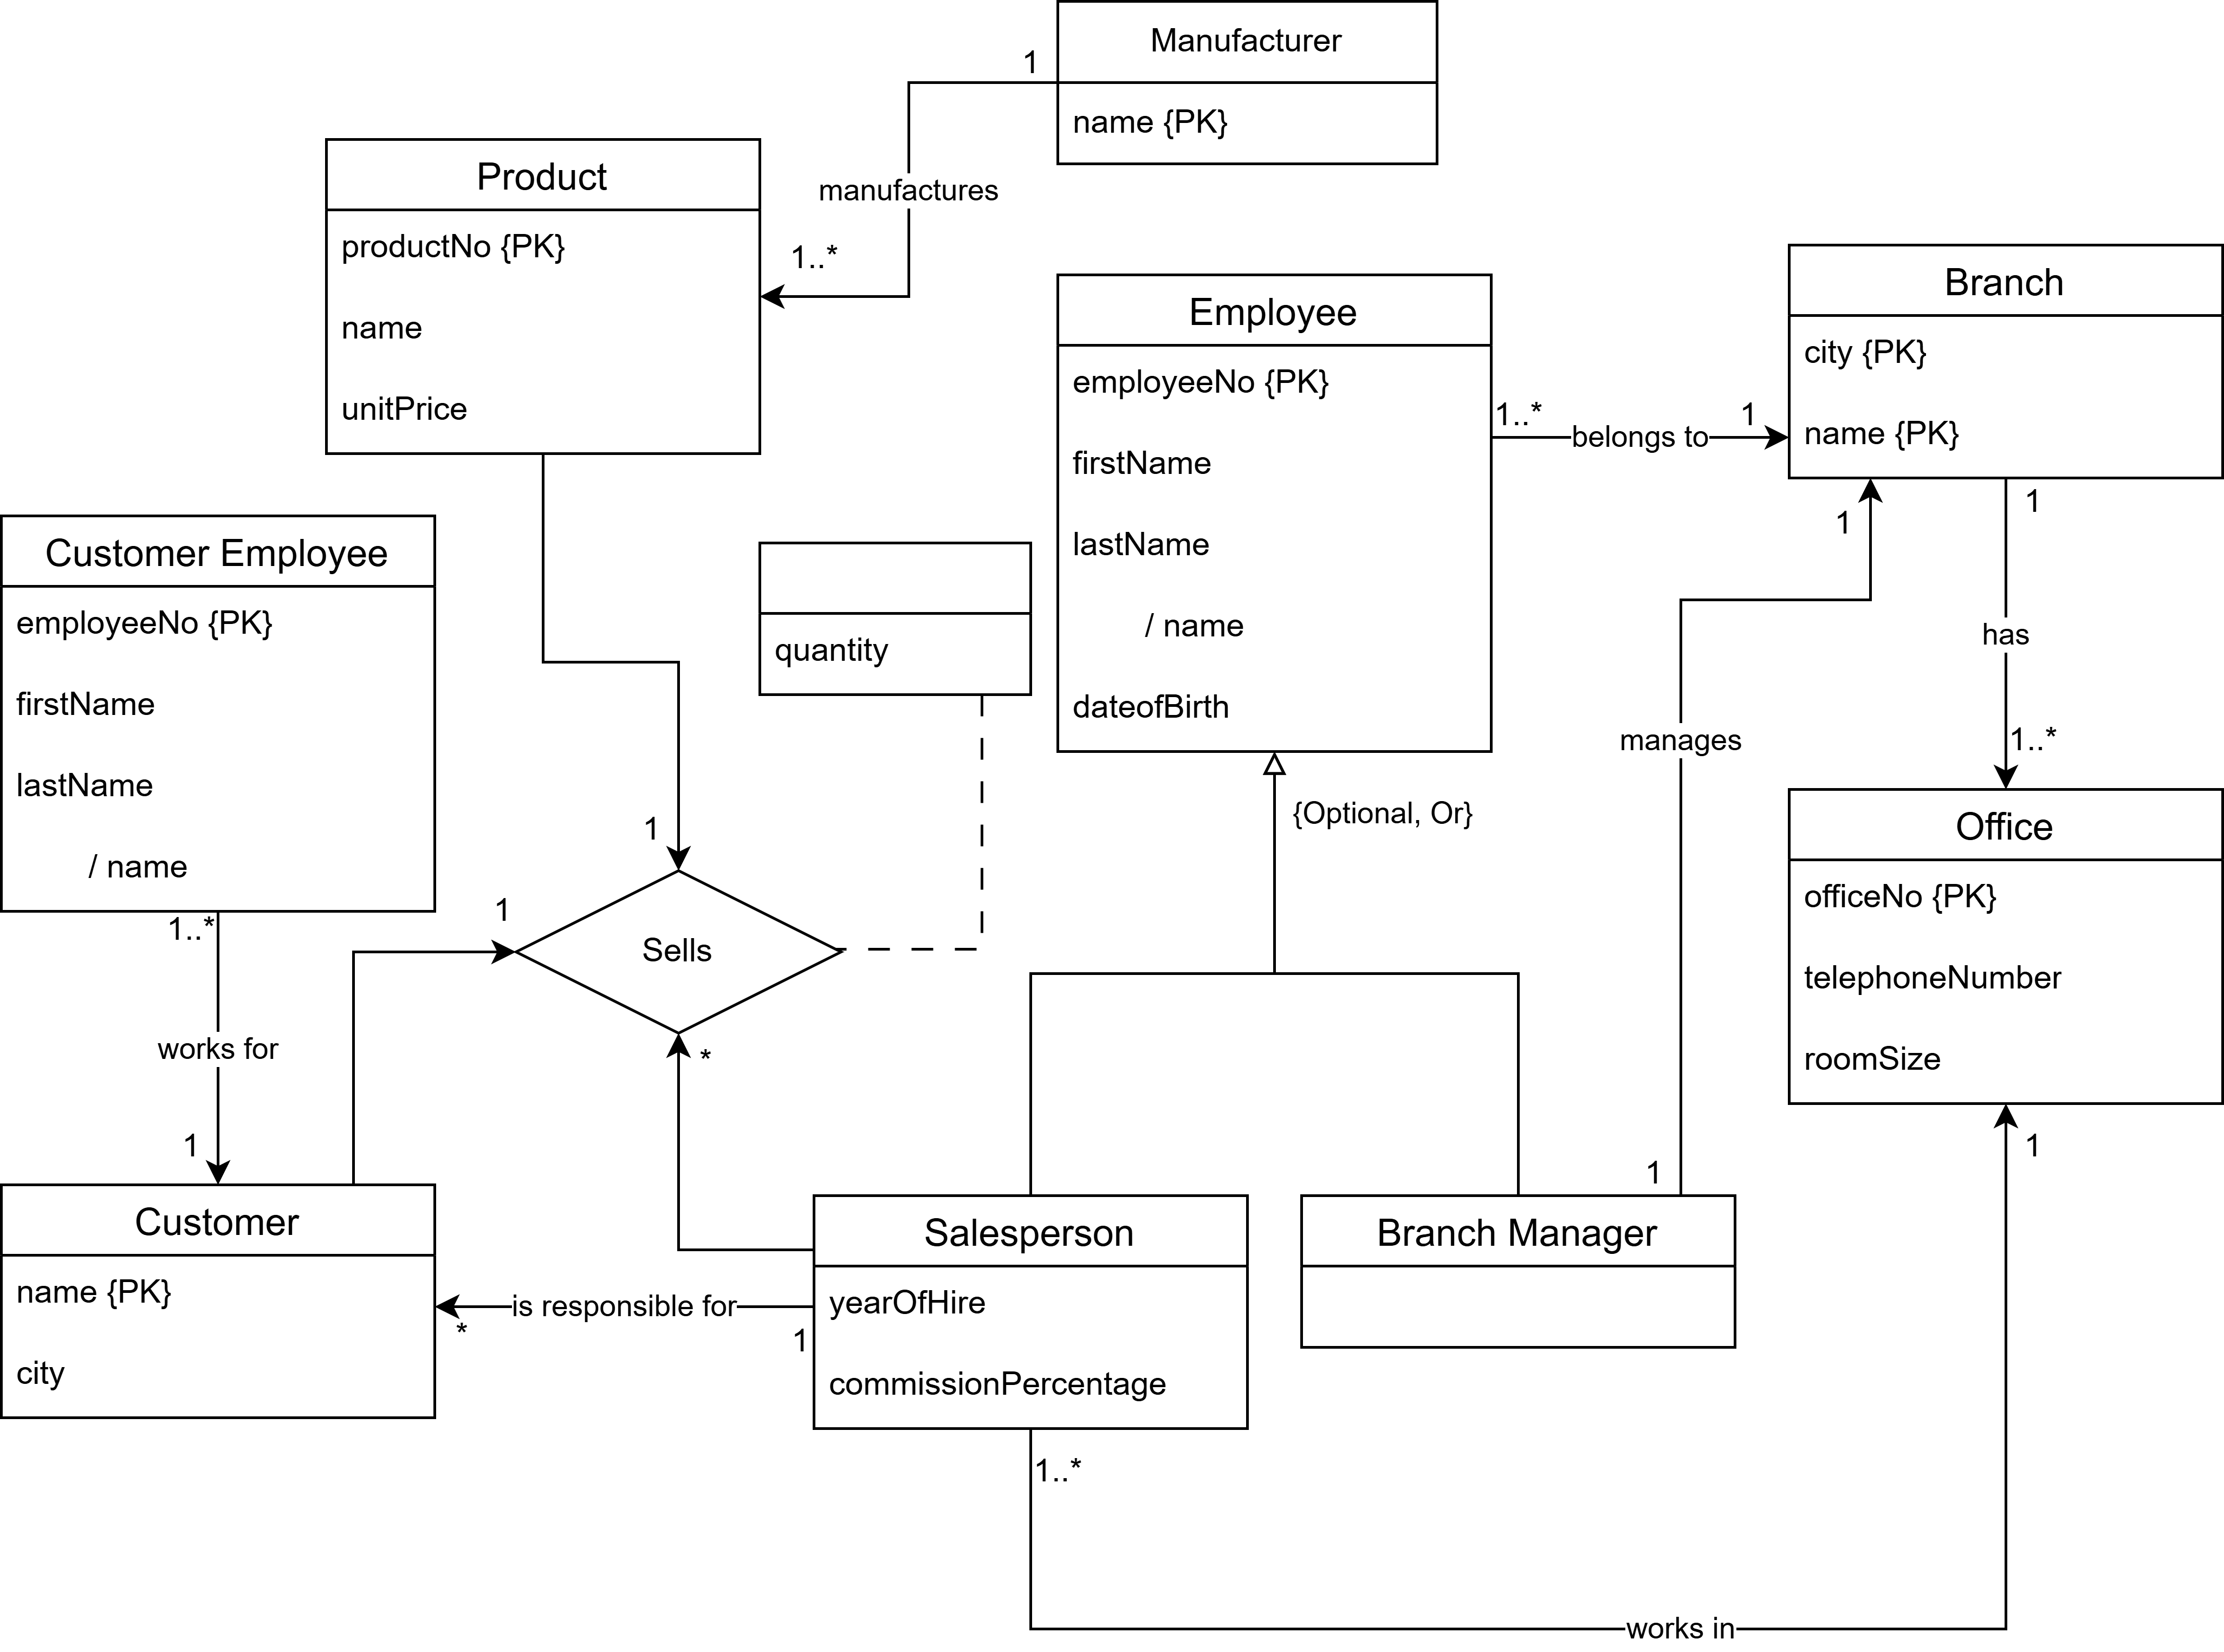
\includegraphics[width=0.8\textwidth]{ER Diagram.png}
    \caption{Entity-Relationship Diagram for C\&E Hardware.}
\end{figure}

\subsection{Explanation}
\subsubsection{The `Branch' and `Office' Tables}
In addition to their city, I also gave \texttt{Branch} a \texttt{name} field to differentiate between branches in the same city. This is because it is possible that a city may have multiple branches, but they would be named differently. The \texttt{city} and \texttt{name} fields then form a composite primary key for the \texttt{Branch} table.

\texttt{officeNo} was an obvious choice for the primary key of the \texttt{Office} table, as it is unique to each office. The \texttt{Office} table additionally has the required attributes for \texttt{telephoneNo} and \texttt{roomSize}.

The \texttt{Branch} table has a `has' relationship with the \texttt{Office} table, with a cardinality of \texttt{1:1..*} because a branch can have many, but at least one, offices, while an office can only belong to one branch.

\subsubsection{The `Employee', `Branch Manager', and `Salesperson' Tables}
I chose to give the \texttt{Employee} a \texttt{employeeNo} for their primary key, as it cannot be guaranteed that all employees in a branch will have unique names. Although only a `salesperson number' is mentioned in the specification, I have assumed that managers and other employees also have unique numbers which can be collectively referred to as \texttt{employeeNo}.

The \texttt{Branch Manager} and \texttt{Salesperson} tables are specialisations of the \texttt{Employee} table, allowing them to share attributes such as \texttt{employeeNo}, \texttt{firstName}, \texttt{lastName}, and \texttt{dateOfBirth}. This specialisation is \texttt{\{Optional, Or\}} because an employee must be either a branch manager, salesperson, or neither.

An \texttt{Employee} has a `works in' relationship with a \texttt{Branch}. This relationship has a cardinality of \texttt{1:1..*} because it is assumed that an employee works in exactly one branch, while a branch can have many (but at least one) employees.

A \texttt{Branch Manager} `manages' exactly one \texttt{Branch}, and a \texttt{Branch} has exactly one \texttt{Branch Manager}. The \texttt{Branch Manager} does not have a relation to a specific \texttt{Office}, as they are assumed to manage the entire branch rather than a specific office.

\subsubsection{The `Customer' Table}
I chose to use \texttt{name} as the primary key for the \texttt{Customer} table, as it should be unique to each \texttt{Customer}. The table also has the required attribute of \texttt{city}. The \texttt{Customer} table has a `has' relationship with the \texttt{Customer Employee} table, with a cardinality of \texttt{1:1..*} because a customer must have at least one employee, but an employee can work for many customers.

The \texttt{Salesperson} table has a `is responsible for' relationship with a \texttt{Customer} with a cardinality of \texttt{1:*} because a salesperson can be responsible for many (including zero) customers, but a customer must have exactly one salesperson.

\subsubsection{The `Customer Employee' Table}
Instead of reusing the \texttt{Employee} table for employees of customers as well as C\&E Hardware, I chose to create a separate \texttt{Customer Employee} table. This is because the data about a customer's employee is only relevant as long as the customer remains a customer of C\&E Hardware, and so by separating the tables, deleting a \texttt{Customer} can cascade to delete all of its employees. This also allows a \texttt{Customer Employee} to have less personal data than a \texttt{Customer}, as such information is not relevant to C\&E Hardware.

A \texttt{customerNo} is assigned to each \texttt{Customer Employee} as their primary key, as it is unique to each employee. The employee's \texttt{firstName} and \texttt{lastName} are also stored in this table.

The \texttt{Customer Employee} table has a `works for' relationship with the \texttt{Customer} table, with a cardinality of \texttt{1:1..*} because an employee must work for a customer, but a customer can have many employees.

\subsubsection{The `Manufacturer' and `Product' Tables}
The \texttt{Product} table has a \texttt{productNo} as its primary key, as it is unique to each product. The table also has the required attributes of \texttt{name} and \texttt{unitPrice}.

The \texttt{Manufacturer} table has a \texttt{name} as its primary key, as it is unique to each manufacturer.

The \texttt{Product} table has a `manufactures' relationship with the \texttt{Manufacturer} table, with a cardinality of \texttt{1:1..*} because a product must be manufactured by a manufacturer, but a manufacturer can manufacture many products.

\subsubsection{The `Sells' Relationship}
There is a three-way relationship between a \texttt{Salesperson}, \texttt{Customer}, and \texttt{Product}. This relationship additionally has an attribute of \texttt{quantity}. I have assumed that a branch or office does not have a specific list of products, but rather that a salesperson can sell any product from any manufacturer. This is why the relationship is between the salesperson and the product, rather than the branch and the product.

The cardinality of the \texttt{Sells} relation is chosen because each relationship must contain exactly one salesperson, one customer, and one product, but a salesperson can sell many products to many customers.

\section{Normalisation}
\subsection{Table Definitions}
\subsubsection{Relational Schema}
The normalised relational schema is as follows:
\begin{lstlisting}
Salesperson(SalespersonNumber, SalespersonName, CommissionPercentage, YearOfHire, DepartmentNumber)
Primary Key: SalespersonNumber
Foreign Key: DepartmentNumber references Department(DepartmentNumber)

Department(DepartmentNumber, ManagerName)
Primary Key: DepartmentNumber

Product(ProductNumber, ProductName, UnitPrice)
Primary Key: ProductNumber

ProductSale(SalespersonNumber, ProductNumber, Quantity)
Primary Key: SalespersonNumber, ProductNumber
Foreign Key: SalespersonNumber references Salesperson(SalespersonNumber), ProductNumber references Product(ProductNumber)
\end{lstlisting}
\subsubsection{Relational Instances}
The relational instances are given in tables \ref{tab:salesperson}, \ref{tab:department}, \ref{tab:product}, and \ref{tab:productsale}; where the primary key is in underlined and foreign keys are in italics\footnote{Some attribute names have been shortened from those given in the schema.}.

\begin{table}[H]
    \centering
    \begin{tabular}{ccccc}
        \toprule
        \textbf{\underline{SalespersonNo}} & \textbf{SalespersonName} & \textbf{CommissionPcnt} & \textbf{YrOfHire} & \textbf{\textit{DeptNo}} \\
        \midrule
        37                                 & Baker                    & 10                      & 2015              & 73                             \\
        86                                 & Adams                    & 15                      & 2011              & 59                             \\
        14                                 & Johnson                  & 10                      & 2018              & 59                             \\
        61                                 & Davies                   & 20                      & 2011              & 59                             \\
        \bottomrule
    \end{tabular}
    \caption{The \texttt{Salesperson} instance.}
    \label{tab:salesperson}
\end{table}

\begin{table}[H]
    \centering
    \begin{tabular}{cc}
        \toprule
        \textbf{\underline{DeptNo}} & \textbf{ManagerName} \\
        \midrule
        73                                & Scott                \\
        59                                & Lopez                \\
        \bottomrule
    \end{tabular}
    \caption{The \texttt{Department} instance.}
    \label{tab:department}
\end{table}

\begin{table}[H]
    \centering
    \begin{tabular}{ccc}
        \toprule
        \textbf{\underline{ProductNo}} & \textbf{ProductName} & \textbf{UnitPrice} \\
        \midrule
        6722                           & Pliers               & 11.50              \\
        4013                           & Saw                  & 26.25              \\
        9440                           & Hammer               & 17.50              \\
        6386                           & Wrench               & 12.95              \\
        1765                           & Drill                & 32.99              \\
        \bottomrule
    \end{tabular}
    \caption{The \texttt{Product} instance.}
    \label{tab:product}
\end{table}

\begin{table}[H]
    \centering
    \begin{tabular}{ccc}
        \toprule
        \textbf{\underline{\textit{ProductNo}}} & \textbf{\underline{\textit{SalespersonNo}}} & \textbf{Quantity} \\
        \midrule
        6722                                    & 37                                          & 688               \\
        4013                                    & 37                                          & 170               \\
        9440                                    & 37                                          & 473               \\
        6386                                    & 86                                          & 1745              \\
        9440                                    & 86                                          & 2529              \\
        1765                                    & 86                                          & 1962              \\
        4013                                    & 86                                          & 3071              \\
        1765                                    & 14                                          & 809               \\
        6722                                    & 14                                          & 734               \\
        6386                                    & 61                                          & 3729              \\
        1765                                    & 61                                          & 3110              \\
        6722                                    & 61                                          & 2738              \\
        \bottomrule
    \end{tabular}
    \caption{The \texttt{ProductSale} instance.}
    \label{tab:productsale}
\end{table}

\subsection{Explanation}
The original table uses the schema:
\begin{lstlisting}
SalesRecords(SalespersonNumber, ProductNumber, SalespersonName, CommissionPercentage, YearOfHire, DepartmentNumber, ManagerName, ProductName, UnitPrice, Quantity)
Primary Key: SalespersonNumber
\end{lstlisting}
I began by getting this table into First Normal Form. This requires removing the repeating groups that each row has relating to the product. I did this by creating a new table \texttt{Product}, and storing a foreign key to the \texttt{Salesperson} in the \texttt{Product}. The schema for the tables in First Normal Form is:
\begin{lstlisting}
Salesperson(SalespersonNumber, SalespersonName, CommissionPercentage, YearOfHire, DepartmentNumber, ManagerName)
Primary Key: SalespersonNumber

Product(ProductNumber, SalespersonNumber, ProductName, UnitPrice, Quantity)
Primary Key: ProductNumber, SalespersonNumber
    Alternate Key: ProductName, SalespersonNumber
Foreign Key: SalespersonNumber references Salesperson(SalespersonNumber)
\end{lstlisting}
To get the tables into Second Normal Form, all partial dependencies must be removed. A partial dependency exists in the \texttt{Product} table, as \texttt{Quantity} only depends on \texttt{SalespersonNumber}, and not on the entire primary key (and the opposite is true for the other attributes). I therefore created a new \texttt{ProductSale} table, resulting in the following schema:
\begin{lstlisting}
Salesperson(SalespersonNumber, SalespersonName, CommissionPercentage, YearOfHire, DepartmentNumber, ManagerName)
Primary Key: SalespersonNumber

Product(ProductNumber, ProductName, UnitPrice)
Primary Key: ProductNumber

ProductSale(SalespersonNumber, ProductNumber, Quantity)
Primary Key: SalespersonNumber, ProductNumber
Foreign Key: SalespersonNumber references Salesperson(SalespersonNumber), ProductNumber references Product(ProductNumber)
\end{lstlisting}
Finally, to get the tables into Third Normal Form, all transitive dependencies must be removed. Transitive dependecies existed in the \texttt{Salesperson} table, as \texttt{ManagerName} depends only on \texttt{DepartmentNumber}, which is not part of the primary key. I therefore created a new \texttt{Department} table, resulting in the following schema:
\begin{lstlisting}
Salesperson(SalespersonNumber, SalespersonName, CommissionPercentage, YearOfHire, DepartmentNumber)
Primary Key: SalespersonNumber
Foreign Key: DepartmentNumber references Department(DepartmentNumber)

Department(DepartmentNumber, ManagerName)
Primary Key: DepartmentNumber

Product(ProductNumber, ProductName, UnitPrice)
Primary Key: ProductNumber

ProductSale(SalespersonNumber, ProductNumber, Quantity)
Primary Key: SalespersonNumber, ProductNumber
Foreign Key: SalespersonNumber references Salesperson(SalespersonNumber), ProductNumber references Product(ProductNumber)
\end{lstlisting}

\end{document}
